% AI6102 Team Project Report -- Titanic: Machine Learning from Disaster
% Layout follows the spirit of the CVPR author kit (two columns, 10pt Times).
\documentclass[10pt,twocolumn,letterpaper]{article}
\usepackage[letterpaper,top=1in,bottom=1in,left=0.8125in,right=0.8125in,columnsep=0.3125in]{geometry}
\usepackage{times}
\usepackage[T1]{fontenc}
\usepackage{microtype}
\usepackage{graphicx}
\usepackage{booktabs}
\usepackage{array}
\usepackage{multirow}
\usepackage{amsmath,amssymb}
\usepackage[table]{xcolor}
\usepackage[font=small,labelfont=bf,skip=4pt]{caption}
\usepackage{enumitem}
\usepackage{titlesec}
\usepackage[colorlinks=true,linkcolor=blue!50!black,citecolor=blue!50!black,urlcolor=blue!50!black]{hyperref}

\titleformat{\section}{\normalfont\large\bfseries}{\thesection.}{0.5em}{}
\titleformat{\subsection}{\normalfont\normalsize\bfseries}{\thesubsection.}{0.5em}{}
\titlespacing*{\section}{0pt}{8pt}{4pt}
\titlespacing*{\subsection}{0pt}{6pt}{3pt}
\setlist{nosep,leftmargin=*}
\newcommand{\fillin}[1]{\textcolor{red}{\textbf{[#1]}}}
\newcommand{\pp}{\,pp}
\setlength{\tabcolsep}{4pt}

\begin{document}

\twocolumn[{%
\begin{center}
{\Large\bfseries Titanic Survival Prediction with Leakage-Safe Co-Traveller Features\\[2pt]
and an Honest Reading of a Contaminated Leaderboard\par}
\vspace{10pt}
{\normalsize
JI QIANKUN (G2605301H) \qquad GAN MINGRUI (G2602128C)\\[3pt]
AI6102 Machine Learning Methodologies \& Applications \quad|\quad Kaggle team: \emph{AI6102 Project}\\[2pt]
Competition: \emph{Titanic -- Machine Learning from Disaster} (ongoing, Getting Started)\par}
\vspace{12pt}
\end{center}
}]

\begin{abstract}
\noindent
We predict passenger survival on the Titanic from 891 labelled records and submit predictions for 418 unlabelled passengers to the ongoing Kaggle competition. The project was run as a sequence of pre-registered, controlled experiments: every preprocessing statistic is fitted inside the training fold, every comparison reuses the same saved folds, and every selection rule was written into a configuration file before results were seen. Ablations show that the passenger's title is the single most useful engineered feature (+2.6\pp\ for logistic regression) and that survival is strongly correlated within travelling groups. Our final model encodes ticket and family groups as native categorical features in CatBoost, whose ordered target statistics prevent a passenger's own label from leaking into the group encoding. It reaches 84.74\% stratified cross-validation accuracy and a public score of \textbf{0.80382} (336/418 correct), ranked 821 of 11{,}283 teams. We then show that the top of the leaderboard is dominated by submissions that cannot come from a predictive model: 365 teams score exactly 1.00000 and 408 teams score at least 0.85885, separated from all other teams by an empty band of seven passengers. Kaggle community discussions, and a public Kaggle dataset that republishes the test set with its true labels, show that the full answer key can be recovered by matching test passengers' names to historical passenger records; we therefore regard these scores as label lookup, not prediction. Excluding them, our honest rank is about 413 of 10{,}875 (top 3.8\%); even the raw rank is inside the top 10\%. We never used external labels or edited any prediction by hand.
\end{abstract}

%=====================================================================
\section{Problem Statement}
%=====================================================================
The task is binary classification. Each row describes one passenger by ticket class (\texttt{Pclass}), name, sex, age, numbers of siblings/spouses (\texttt{SibSp}) and parents/children (\texttt{Parch}) aboard, ticket number, fare, cabin and port of embarkation. The target \texttt{Survived} is 1 if the passenger survived. Kaggle provides 891 labelled training passengers and 418 test passengers whose labels are hidden; a submission is a two-column file (\texttt{PassengerId}, \texttt{Survived}) scored by accuracy. The leaderboard page states that it is ``calculated with all of the test data'', so there is no separate private split, and one passenger changes the score by $1/418 = 0.239$ percentage points (pp).

Our aim was not only a good score but a result we can defend: a reproducible pipeline whose reported gains are supported by controlled experiments, and an honest account of what the leaderboard does and does not measure.

%=====================================================================
\section{Challenges}
%=====================================================================
\textbf{Small data and coarse metrics.} A validation fold holds about 178 passengers, so one passenger moves fold accuracy by 0.56\pp. Differences below about 1\pp\ are within the noise of a single split, which makes model selection fragile.

\textbf{Missing values.} In training, \texttt{Age} is missing for 177 passengers (19.9\%), \texttt{Cabin} for 687 (77.1\%) and \texttt{Embarked} for 2. In the test set, \texttt{Age} is missing for 86, \texttt{Cabin} for 327 and \texttt{Fare} for one passenger, so the pipeline must handle a column that is complete in training.

\textbf{Strong but entangled signals.} Overall survival is 38.4\% (342/891). Sex and class dominate (Fig.~\ref{fig:eda}): 74.2\% of women but only 18.9\% of men survived, and the female rate falls from 96.8\% in first class to 50.0\% in third. Age, family size and fare interact with these effects, and some subgroups are tiny.

\textbf{Dependence between passengers.} Families and companions shared tickets and often shared a fate. In training, 344 passengers share a ticket with another training passenger, and 115 ticket values appear in both files, covering 152 of the 418 test passengers. A random split therefore lets a model ``see'' a validation passenger's companions, which is optimistic for passengers travelling alone but realistic for the Kaggle test set. Using this structure without leaking labels is the central modelling problem.

\textbf{Selection bias.} Reusing the same folds for many decisions, and receiving leaderboard feedback, slowly turns the validation data into training data for the researcher~\cite{cawley2010,blum2015}.

\textbf{A contaminated leaderboard.} The real outcome of every passenger is public historical record, and the Kaggle community openly describes looking test passengers up by name. A leaderboard position can therefore reflect answer lookup rather than learning (Sec.~\ref{sec:leaderboard}).

\begin{figure}[t]
\centering
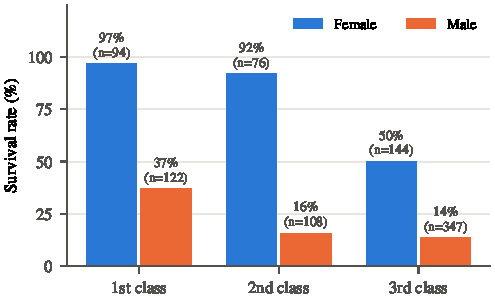
\includegraphics[width=\linewidth]{figures/eda_sex_class.pdf}
\caption{Survival rate by sex and ticket class in the training set. Sex and class explain much of the outcome, but within-class differences remain large.}
\label{fig:eda}
\end{figure}

%=====================================================================
\section{Proposed Solution}
%=====================================================================
\subsection{Motivation}
We framed four hypotheses that the experiments in Sec.~\ref{sec:exp} test directly.
\begin{enumerate}[label=\textbf{H\arabic*}]
\item \textbf{Social role.} The title in the name (Mr, Mrs, Miss, Master, \dots) summarises sex, age group and status together, and should help more than the raw fields alone. ``Master'' in particular identifies boys whose age may be missing.
\item \textbf{Informative missingness.} Whether a cabin was recorded is linked to class and record-keeping, so the indicator itself may carry signal.
\item \textbf{Group survival.} Under ``women and children first'', families and ticket companions tended to survive or perish together. Knowing how a passenger's co-travellers fared in training should therefore help predict their own outcome.
\item \textbf{Leakage-safe encoding.} Group identifiers have very high cardinality. Naive target encoding includes a passenger's own label in their group statistic, which inflates validation scores. An encoding that excludes a row's own label should keep the gain from H3 without the leak.
\end{enumerate}

\subsection{Final pipeline (v7)}
\textbf{Features.} From the raw columns we derive the following, row by row, with no train--test concatenation:
\begin{itemize}
\item \emph{Raw:} Age, Fare, SibSp, Parch, Pclass, Sex, Embarked.
\item \emph{Title:} extracted from Name and mapped to Mr, Mrs, Miss, Master, Officer (Capt, Col, Major, Dr, Rev) or Royalty (Sir, Lady, Countess, \dots); Mme/Ms$\to$Mrs, Mlle$\to$Miss.
\item \emph{Deck:} first letter of Cabin, or U if missing (this subsumes the cabin-missing indicator).
\item \emph{TicketPrefix:} first non-numeric token of the ticket, else XXX.
\item \emph{Family:} FamilySize $=$ SibSp $+$ Parch $+$ 1, with Singleton, Small (2--4) and Large ($\geq$5) indicators.
\item \emph{Group keys:} TicketGroup (normalised ticket string) and FamilyGroupKey (upper-case surname $+$ family size). Passengers travelling alone get a unique key, so they are not pooled into one artificial group.
\end{itemize}

\textbf{Imputation} uses only the training partition: Age by the median of its (Sex, Pclass, Title) cell, falling back to (Sex, Pclass) and then the global median; Fare by the training mean; Embarked by ``S''.

\textbf{Model.} CatBoost~\cite{catboost} with depth 4, 600 iterations, learning rate 0.035, L2 regularisation 5, \emph{ordered} boosting and seed 42. The categorical features are Pclass, Embarked, Deck, Title, TicketPrefix, TicketGroup and FamilyGroupKey. We use no early stopping (so validation rows never influence training) and a fixed 0.5 threshold.

\textbf{Why this satisfies H3--H4.} CatBoost replaces each categorical value with a target statistic computed over a random permutation, using only the rows that come \emph{before} the current row. A passenger's own label never enters their encoding, and the permutation is resampled across trees. A test passenger whose ticket or family appears in training inherits a statistic learned from those companions; an unseen group falls back to the prior. This is exactly the behaviour H3 asks for, without the self-leakage H4 warns about.

\textbf{Engineering safeguards.} Each experiment has a frozen configuration, a separate output directory, saved fold assignments, out-of-fold (OOF) predictions, code and data hashes, unit tests (for example, that features never read the target and are unchanged by other rows) and an independent verification script that reloads every saved fold model and reproduces its predictions.

%=====================================================================
\section{Experiments}\label{sec:exp}
%=====================================================================
\subsection{Protocol}
We fixed two five-fold schemes with seed 42 and saved them by \texttt{PassengerId}: \emph{stratified} folds (the primary metric) and \emph{ticket-group} folds (\texttt{StratifiedGroupKFold}), in which no ticket crosses the train/validation boundary. The group scheme stress-tests performance on passengers whose companions are unseen. Later rounds added a fresh-seed stratified scheme (seed 20261117) and connected-component group folds, where tickets and families linked by any shared key stay together. Nested CV (inner three folds for selection, outer five for evaluation) was used in v3/v4 and v13. We report mean fold accuracy. Fold standard deviation describes variation and is not a confidence interval. In total the project ran more than 2{,}000 cross-validation fits, and every candidate, including the failures, is kept.

\subsection{Verifying the motivations}
\textbf{H2 (missingness).} Starting from a logistic-regression (LR) baseline on the seven raw fields (79.69\% stratified / 80.03\% grouped), adding four missing-value indicators gave +0.56\pp\ in both schemes. A leave-one-in/leave-one-out ablation (Table~\ref{tab:h2}) attributes the whole gain to the Cabin indicator: it adds five correct OOF predictions on its own, and removing it from the bundle loses seven. The Fare indicator is constant in training and does nothing. FamilySize alone changed one prediction, as expected for a linear model, since it is a linear combination of existing inputs.

\begin{table}[t]
\centering\small
\caption{Missing-indicator ablation with LR (accuracy change in pp, same folds). ``Only'': flag added to the no-flag model. ``Drop'': flag removed from the all-flag model.}
\label{tab:h2}
\begin{tabular}{lrrrr}
\toprule
 & \multicolumn{2}{c}{Only vs.\ none} & \multicolumn{2}{c}{Drop vs.\ all}\\
\cmidrule(lr){2-3}\cmidrule(lr){4-5}
Indicator & Strat. & Group & Strat. & Group\\
\midrule
Age      & $-0.22$ & $-0.11$ & $-0.00$ & $+0.00$\\
Fare     & $0.00$ & $0.00$ & $0.00$ & $0.00$\\
Embarked & $+0.11$ & $0.00$ & $0.00$ & $0.00$\\
\textbf{Cabin} & $\mathbf{+0.56}$ & $\mathbf{+0.56}$ & $\mathbf{-0.78}$ & $\mathbf{-0.67}$\\
\bottomrule
\end{tabular}
\end{table}

\textbf{H1 (title).} Table~\ref{tab:h1} adds or removes one module at a time from an LR model. Title is by far the strongest single addition (+2.58\pp\ stratified, +2.92\pp\ grouped), and removing it from the full model costs 2.36\pp. The Sex$\times$Class interaction also matters, while Deck is context-dependent: dropping it raises stratified accuracy but lowers grouped accuracy.

\begin{table}[t]
\centering\small
\caption{LR feature ablation (mean 5-fold accuracy, \%). ``basic'' = raw fields + Cabin flag. ``full'' = basic + Title, family features, Sex$\times$Class, Deck, AgeMissing and log-fare.}
\label{tab:h1}
\begin{tabular}{lrr}
\toprule
LR feature set & Stratified & Ticket-group\\
\midrule
basic & 80.25 & 80.70\\
basic + Title & \textbf{82.83} & \textbf{83.62}\\
basic + family features & 81.71 & 81.60\\
basic + Sex$\times$Class & 81.03 & 81.26\\
\midrule
full & 83.61 & 84.29\\
full $-$ Title & 81.26 & 81.37\\
full $-$ Sex$\times$Class & 82.94 & 83.39\\
full $-$ Deck & 83.95 & 83.85\\
\bottomrule
\end{tabular}
\end{table}

\textbf{Model family on fixed features.} With identical inputs (raw fields + Cabin flag) and identical folds, nonlinear models beat LR (Table~\ref{tab:models}). The predefined 50/50 RF/HGB blend scored best and became our first submission (v1).

\begin{table}[t]
\centering\small
\caption{Estimators on the same 13 encoded inputs and folds (accuracy, \%; SD in pp).}
\label{tab:models}
\begin{tabular}{lrrr}
\toprule
Model & Strat. (SD) & Group & AUC\\
\midrule
Logistic regression & 80.25 (2.74) & 80.59 & 0.855\\
RF, depth 6 & 82.49 (1.94) & 81.82 & 0.870\\
RF, min leaf 3 & 82.94 (1.53) & 81.93 & 0.878\\
HGB, 7 leaves & 83.50 (2.48) & 82.16 & 0.875\\
HGB, 15 leaves & 83.84 (3.40) & 80.93 & 0.876\\
\textbf{RF + HGB blend (v1)} & \textbf{83.95} (3.30) & \textbf{82.49} & \textbf{0.881}\\
\bottomrule
\end{tabular}
\end{table}

\textbf{H3 (group survival) and H4 (encoding).} We first added cross-fitted target encodings of TicketGroup and FamilyGroupKey to a fixed random-forest recipe (v5 $\to$ v6). Encodings for the training rows were produced by an inner five-fold cross-fit, so no passenger saw their own label. RF improved from 82.94\% to 84.29\% stratified, while grouped accuracy moved only from 82.49\% to 82.05\%. HGB with the same encoding collapsed to 78.34\% grouped, a sign that it memorised group rates. Table~\ref{tab:cat} then compares encodings inside CatBoost. Native ordered statistics (\texttt{cb\_groups\_d4}) give the best balance: +1.12\pp\ stratified and +2.02\pp\ on the fresh seed over the same model without groups, while losing only 0.23\pp\ in the grouped scheme. Explicit cross-fitted encoding scores similarly on random splits but loses 1.91\pp\ on unseen groups. This supports both H3 (group information helps when companions are seen, as for 152 test passengers) and H4 (how it is encoded decides whether it generalises). The pre-declared rule (stratified average at least +0.5\pp\ above the v6 RF, grouped drop at most 0.5\pp) selected \texttt{cb\_groups\_d4}. One blend reached 85.07\% on a single split but was rejected because its other checks were weaker.

\begin{table}[t]
\centering\small
\caption{v7 CatBoost comparison (accuracy, \%). S1: original stratified, S2: fresh-seed stratified, G: ticket-group.}
\label{tab:cat}
\begin{tabular}{lrrrc}
\toprule
Configuration & S1 & S2 & G & Pass\\
\midrule
v6 RF + peer TE (ref.) & 84.29 & 83.28 & 82.05 & ref.\\
CB, no group keys & 83.61 & 82.38 & \textbf{82.16} & no\\
\rowcolor{blue!6}\textbf{CB, native groups, d4} & 84.74 & \textbf{84.40} & 81.93 & \textbf{yes}\\
CB, native groups, d6 & 84.51 & 83.17 & 81.27 & no\\
CB, cross-fit TE, d4 & \textbf{84.85} & 83.84 & 80.25 & no\\
RF + CB groups d4 (50/50) & 84.62 & 84.18 & 82.05 & yes\\
RF + CB groups d6 (50/50) & 85.07 & 83.39 & 81.38 & no\\
\bottomrule
\end{tabular}
\end{table}

\subsection{Leaderboard results}
Table~\ref{tab:subs} lists the seven distinct models we scored on Kaggle. The best, v7, scored \textbf{0.80382}, i.e.\ 336 of 418 passengers correct, with 146 predicted survivors. Fig.~\ref{fig:cvlb} shows a consistent CV-to-leaderboard gap of 4.4--9.2\pp. Across these seven models the rank correlation between CV and leaderboard accuracy is only $\rho=0.57$: higher CV did not reliably mean a higher public score. Two lessons follow. First, the largest leaderboard gains (v5$\to$v6 +1.67\pp, v6$\to$v7 +0.72\pp) came from the group features motivated by H3, which match the train--test overlap of the real test set. Second, gains on reused folds did not transfer: v4 had high selection CV but the worst score, and the v12 exploratory model had the highest CV (85.02\%) yet scored 1.20\pp\ below v7.

\begin{table}[t]
\centering\small
\caption{Models scored on Kaggle. CV = stratified 5-fold mean (v12: average of two stratified schemes); Group = ticket-group CV.}
\label{tab:subs}
\setlength{\tabcolsep}{3pt}
\begin{tabular}{llrrr}
\toprule
Ver. & Model & CV & Group & Kaggle\\
\midrule
v1 & RF+HGB blend, raw + Cabin & 83.95 & 82.49 & 0.77033\\
v2 & LR, full features & 83.61 & 84.29 & 0.76076\\
v4 & HGB 7-leaf, no Deck & 84.29 & -- & 0.75119\\
v5 & RF recipe (title, prefix) & 82.94 & 82.49 & 0.77990\\
v6 & v5 + cross-fit peer TE & 84.29 & 82.05 & 0.79665\\
\rowcolor{blue!6}\textbf{v7} & \textbf{CatBoost, native groups} & 84.74 & 81.93 & \textbf{0.80382}\\
v12 & role-group blend (exploratory) & 85.02 & 81.93 & 0.79186\\
\bottomrule
\end{tabular}
\end{table}

\begin{figure}[t]
\centering
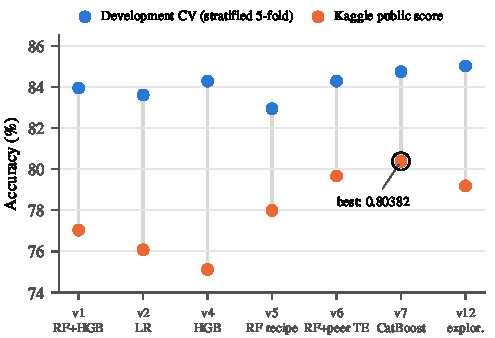
\includegraphics[width=\linewidth]{figures/cv_vs_kaggle.pdf}
\caption{Development CV vs.\ public score for every submission. The gap is 4.4--9.2\pp, and CV order is a weak guide to leaderboard order.}
\label{fig:cvlb}
\end{figure}

\begin{figure}[t]
\centering
\IfFileExists{figures/leaderboard_screenshot.png}{%
  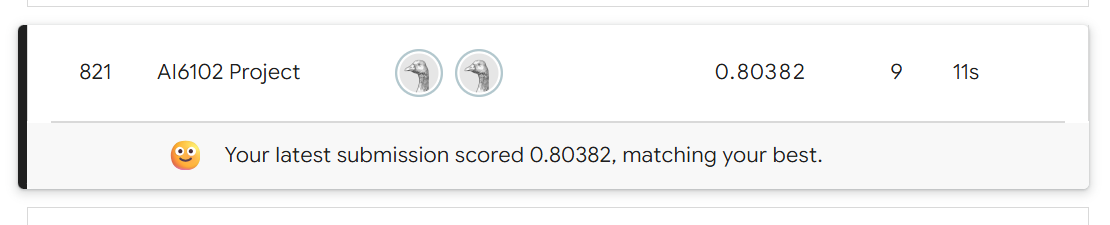
\includegraphics[width=\linewidth]{figures/leaderboard_screenshot.png}%
}{%
  \fbox{\parbox[c][1.3in][c]{0.94\linewidth}{\centering\color{red}\bfseries
  [Insert leaderboard screenshot of the 0.80382 submission here:\\ save it as \texttt{figures/leaderboard\_screenshot.png} and recompile]}}%
}
\caption{Kaggle leaderboard screenshot of our team \emph{AI6102 Project}: public score 0.80382 (v7), rank 821, nine entries.}
\label{fig:screenshot}
\end{figure}

\subsection{Experiments that did not help}
After v7 we ran six more pre-registered rounds (v8--v13, nearly 480 fits). None was adopted:
\begin{itemize}
\item \textbf{v8} conditional peer features: stratified average 84.51\% ($<$ v7's 84.57\%).
\item \textbf{v9} ticket-count, fare-per-person and interaction features: +0.17\pp, below the +0.5\pp\ gate.
\item \textbf{v10} seed averaging, regularised and native-missing variants, and \emph{soft routing} (use v7 when a passenger has known companions, otherwise average with a no-group model): +0.17\pp\ stratified, +0.90\pp\ grouped, still below the gate.
\item \textbf{v11} new connected-component folds and fallback experts (ExtraTrees, calibrated SVM): routing gained one passenger on 891.
\item \textbf{v12} woman/child-vs-adult-male role groups: 85.02\% stratified, but the grouped gate failed. An exploratory export scored 0.79186 on Kaggle.
\item \textbf{v13} LightGBM~\cite{lightgbm} with nested selection: the selection \emph{procedure} gained +0.34\pp\ on outer folds, but on all 891 rows the inner rule still chose v7 (83.39\% vs.\ 82.94\% for the best alternative), so no new model was exported.
\end{itemize}
These negative results matter: they show that the remaining gains we could find were within fold noise, and that our pre-registered gates stopped us from chasing them on the leaderboard.

%=====================================================================
\section{How Much Does the Leaderboard Rank Mean?}\label{sec:leaderboard}
%=====================================================================
On 18 November 2026 (02:43 UTC) we recorded the full public leaderboard: 11{,}283 ranked teams plus the ``Assume All Perished'' benchmark (0.62200). We stored score counts only, no team identities. Fig.~\ref{fig:lb} shows the distribution.

\begin{figure*}[t]
\centering
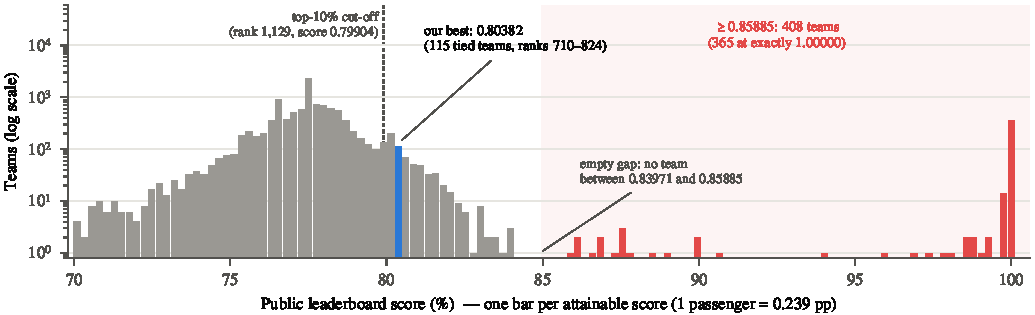
\includegraphics[width=\textwidth]{figures/leaderboard_distribution.pdf}
\caption{Public leaderboard score distribution (18 Nov 2026, scores $\geq$ 0.70, log scale). Honest scores decline steadily up to 0.83971; after an empty band of seven passengers, a second mass of 408 teams rises to 365 perfect scores (red).}
\label{fig:lb}
\end{figure*}

\textbf{The answer key is public.} The Titanic test labels are not secret. The complete list of 1{,}309 passengers with their survival status, i.e.\ the 891 training plus the 418 test passengers, has long been distributed as a standard dataset compiled mainly from Encyclopedia Titanica~\cite{openml,et}. Kaggle's own community documents how this is used. In a Titanic discussion thread asking how teams reach 100\%, the most up-voted reply explains that they take the survivor list from Encyclopedia Titanica and join it to \texttt{test.csv} on the passenger's name and other columns~\cite{kagglediscuss}. A public Kaggle dataset goes further: it republishes \texttt{test.csv} with the true labels retrieved from that historical source, and its author reports that the labels were ``validated by getting a 1.0 score in the competition''~\cite{howe}. A perfect submission therefore needs no learning at all; matching each test passenger's name against the historical record is enough. This is a textbook case of target leakage~\cite{kaufman2012}.

\textbf{The leaderboard shows the footprint of this lookup.} Four observations in the score distribution agree with the community reports.
\begin{enumerate}
\item \emph{Perfect scores.} 365 teams score exactly 1.00000, 382 score at least 0.99, and 393 score at least 0.90. A perfect score requires predicting all 418 passengers correctly, including many whose features look like those of passengers who had the opposite fate.
\item \emph{A bimodal top.} Below 0.84 the counts decline steadily as the score rises (68, 51, 48, 33, 34, 20, 15, 9, \dots, 3 teams at 0.83971). Then \emph{no} team scores between 0.83971 (351/418) and 0.85885 (359/418), and above the gap the counts \emph{increase} again towards 1.0. A single population of models would not produce an empty band of seven passengers followed by a rising tail.
\item \emph{Inverted answer keys.} Eleven teams score exactly 0.00000 and one scores 0.00239. Being wrong on every passenger is as hard as being right on every passenger: it requires knowing every label.
\item \emph{Near-perfect clusters.} Fourteen teams score 0.99760 (one passenger wrong) and a further 13 lie between 0.94 and 0.993. A name lookup with a few matching mistakes, or a looked-up file with a handful of rows changed, produces exactly such scores; a model trained on 891 rows does not.
\end{enumerate}
Taking the public answer key, the community reports and the score distribution together, we regard the 408 submissions at or above 0.85885, and certainly the 365 perfect ones, as obtained by looking up passenger names in the historical record rather than by prediction. For comparison, well-known public solutions that do not use leaked data report scores of around 0.81~\cite{besbes}. Repeated leaderboard probing is a milder form of the same problem~\cite{blum2015}. We judge the aggregate pattern only and name no individual team.

\textbf{Adjusted rank.} Our 0.80382 is shared by 115 teams occupying ranks 710--824 (Kaggle orders tied teams by submission time); our team \emph{AI6102 Project} was ranked 821 in the screenshot of Fig.~\ref{fig:screenshot}, taken on the same day. Table~\ref{tab:rank} removes implausible scores under two thresholds. With the conservative rule (only exact 1.00000 removed), our rank becomes about 456. With the gap-based rule (all 408 teams at $\geq$0.85885 removed), it becomes about 413 of 10{,}875, i.e.\ the top 3.8\%. Even without any adjustment, rank 821 of 11{,}283 (7.3\%) is inside the top 10\%, whose cut-off is rank 1{,}129 (score 0.79904). A re-check at 07:19 UTC the same day found 11{,}312 teams, our team at rank 823 and the tied block at 712--828, with the same 365 perfect and 408 implausible scores. Even at the last place of the tied block (828 of 11{,}312, 7.3\%), our result stays inside the top 10\%. In short, \emph{under every counting rule we considered, raw or adjusted, our rank is within the top 10\%.}

\begin{table}[t]
\centering\small
\caption{Our rank under different treatments of implausible scores (18 Nov 2026: score snapshot at 02:43 UTC, screenshot, and a re-check at 07:19 UTC). Adjusted ranks subtract the removed teams from our rank. The tie block is the range of ranks held by all teams at 0.80382.}
\label{tab:rank}
\begin{tabular}{lrrr}
\toprule
Treatment & Rank & Teams & Top\\
\midrule
Raw leaderboard (our row) & 821 & 11{,}283 & 7.3\%\\
\quad tie block at 0.80382 & 710--824 & & 6.3--7.3\%\\
Remove 365 perfect scores & $\approx$456 & 10{,}918 & 4.2\%\\
\rowcolor{blue!6}Remove 408 scores $\geq$0.85885 & $\approx$\textbf{413} & 10{,}875 & \textbf{3.8\%}\\
\quad tie block at 0.80382 & 302--416 & & 2.8--3.8\%\\
\midrule
Re-check 07:19 UTC, raw & 823 & 11{,}312 & 7.3\%\\
\quad worst case in tie block & 828 & 11{,}312 & 7.3\%\\
\quad remove 408 scores $\geq$0.85885 & $\approx$415 & 10{,}904 & 3.8\%\\
\bottomrule
\end{tabular}
\end{table}

\textbf{Our integrity statement.} We used only the official \texttt{train.csv} and \texttt{test.csv}. No external passenger list, no test label and no hand edit of any prediction entered our pipeline. Kaggle lists nine entries for our team (Fig.~\ref{fig:screenshot}); Table~\ref{tab:subs} covers the seven distinct models whose scores we recorded. The v7 file is byte-identical to the one produced by the saved model (SHA-256 \texttt{97c9b5ae\ldots d40c}). We acknowledge that repeated leaderboard feedback is itself mild adaptation to the test set. We kept it small by deciding candidates with pre-registered CV rules, not by leaderboard probing.

%=====================================================================
\section{Discussion and Limitations}
%=====================================================================
Our cross-validation estimates are optimistic. The labels were explored before modelling, the same folds informed many decisions, and the leaderboard gave repeated feedback. Nested CV in v3/v4 and v13 reduces but does not remove this bias. The persistent 4--5\pp\ CV-to-leaderboard gap of our best models is consistent with that optimism and with the fact that only part of the test set has companions in training. Ticket groups and surname-plus-size keys are imperfect proxies for real travelling parties: unrelated passengers can share a surname, and companions can hold different tickets. The grouped schemes are stress tests, not exact simulations of the Kaggle split. Finally, the leaderboard snapshot is a single moment of a rolling leaderboard, and our adjusted rank depends on the threshold chosen; we therefore report both thresholds and the tie block.

%=====================================================================
\section{Conclusion}
%=====================================================================
What we learned from this competition:
\begin{itemize}
\item \textbf{Domain-driven features beat model tuning.} Title (+2.6\pp) and co-traveller identity gave the largest, most repeatable gains. Swapping or tuning models gave fractions of a point.
\item \textbf{How a feature is encoded can matter as much as the feature.} Group survival is real signal, but naive target statistics leak. CatBoost's ordered statistics kept the gain on random splits and lost the least on unseen groups.
\item \textbf{Validate the way you will be tested, and pre-register decisions.} Grouped, fresh-seed and nested CV, plus fixed selection gates, protected us from several attractive but spurious ``improvements'' (v4, v12) that the leaderboard later confirmed were not real.
\item \textbf{A leaderboard is evidence only if the test labels are secret.} On Titanic they are not: the answer key can be looked up by passenger name, as the Kaggle community itself documents. About 400 entries above us are attributable to this lookup, and our honest standing is roughly rank 413 (top 3.8\%), compared with 821 on the raw board.
\end{itemize}
Our best submission, CatBoost with leakage-safe co-traveller categories, scores 0.80382 using only the competition data.

{\small
\begin{thebibliography}{99}\setlength{\itemsep}{1pt}
\bibitem{kaggle} W.~Cukierski. Titanic -- Machine Learning from Disaster. Kaggle, 2012. \url{https://www.kaggle.com/competitions/titanic}
\bibitem{catboost} L.~Prokhorenkova, G.~Gusev, A.~Vorobev, A.~V.~Dorogush, A.~Gulin. CatBoost: unbiased boosting with categorical features. In \emph{NeurIPS}, 2018.
\bibitem{lightgbm} G.~Ke \emph{et al.} LightGBM: A highly efficient gradient boosting decision tree. In \emph{NeurIPS}, 2017.
\bibitem{sklearn} F.~Pedregosa \emph{et al.} Scikit-learn: Machine learning in Python. \emph{JMLR}, 12:2825--2830, 2011.
\bibitem{cawley2010} G.~C.~Cawley, N.~L.~C.~Talbot. On over-fitting in model selection and subsequent selection bias in performance evaluation. \emph{JMLR}, 11:2079--2107, 2010.
\bibitem{blum2015} A.~Blum, M.~Hardt. The Ladder: A reliable leaderboard for machine learning competitions. In \emph{ICML}, 2015.
\bibitem{kaufman2012} S.~Kaufman, S.~Rosset, C.~Perlich, O.~Stitelman. Leakage in data mining: Formulation, detection, and avoidance. \emph{ACM TKDD}, 6(4), 2012.
\bibitem{kagglediscuss} K.~Sharma and commenters. How people are achieving 100\% accuracy in Titanic ML competition? Kaggle discussion, 2020. \url{https://www.kaggle.com/discussions/general/214175}
\bibitem{howe} W.~Howe. Titanic -- Labelled Test Set. Kaggle dataset, 2023. \url{https://www.kaggle.com/datasets/wesleyhowe/titanic-labelled-test-set}
\bibitem{openml} F.~E.~Harrell Jr., T.~Cason. Titanic dataset (1{,}309 passengers with survival status). OpenML data ID 40945, 2017. \url{https://www.openml.org/d/40945}
\bibitem{et} Encyclopedia Titanica. Titanic survivors. \url{https://www.encyclopedia-titanica.org/titanic-survivors/}
\bibitem{besbes} A.~Besbes. How to score 0.8134 in Titanic Kaggle Challenge. GitHub, 2016. \url{https://github.com/ahmedbesbes/How-to-score-0.8134-in-Titanic-Kaggle-Challenge}
\end{thebibliography}
}


\appendix
\section*{Appendix A. Experiment log}
Every round was configured before it was run and kept, including failures. Fits count cross-validation model fits (nested rounds include inner fits). Accuracies are stratified 5-fold means unless noted.

{\footnotesize
\begin{tabular}{@{}l>{\raggedright\arraybackslash}p{3.45cm}r>{\raggedright\arraybackslash}p{2.05cm}@{}}
\toprule
Round & Question & Fits & Outcome\\
\midrule
base & Dummy vs.\ LR, two fold schemes & 20 & LR 79.69\%\\
feat & FamilySize, missing flags, log-fare & 40 & flags +0.56\pp\\
abl. & each missing flag in/out & 100 & Cabin flag only\\
v1 & 5 estimators + fixed blend & 50 & 83.95\%; LB 0.77033\\
v2 & Title, family, full sets; LR/RF/HGB & 120 & LB 0.76076\\
v3/v4 & LR ablation; nested selection & 1{,}077 & Title strongest; LB 0.75119\\
v5 & public RF recipe, fold-safe & 60 & 82.94\%; LB 0.77990\\
v6 & cross-fit peer target encoding & 40 & 84.29\%; LB 0.79665\\
\rowcolor{blue!6}v7 & CatBoost group encodings & 65 & 84.74\%; \textbf{LB 0.80382}\\
v8 & conditional peer features & 30 & gate failed\\
v9 & ticket/fare interactions & 30 & gate failed\\
v10 & seeds, routing, regularisation & 60 & gate failed\\
v11 & component folds, fallback experts & 50 & gate failed\\
v12 & role groups, population counts & 80 & gate failed; LB 0.79186\\
v13 & LightGBM, nested selection & 229 & kept v7\\
\midrule
 & Total & 2{,}051 & \\
\bottomrule
\end{tabular}
}

\vspace{4pt}
\noindent\textbf{Reproducibility.} Python 3.11, scikit-learn 1.4.1, CatBoost 1.2.8, LightGBM 4.6.0 (CPU). Configurations, fold assignments, OOF predictions, model files, code snapshots, hashes and verification scripts are stored per round in the project folder. The leaderboard snapshot (score counts only) is in \texttt{outputs/leaderboard\_snapshot\_20261118/}.

\end{document}
